
\documentclass{article}

\usepackage{graphicx}

\begin{document}

		\title{A REPORT ABOUT SMART PHONES POSSESSED BY  MAKERERE UNIVERSITY STUDENTS}
		\author{Author :   MUBANGIZI KINGEDWARD }
		\date{Student No: 213021116}
                      \date{Reg no: 13/U/8200/PS}
		\maketitle
	

	\tableofcontents

\section{ABSTRACT}
This report contains information of favorite smartphones for some Makerere University students studying different courses . Data is taken randomly from any student found either in the University or Outside the boundaries of the University. Further, the records are inserted into a database through internet to a sever which is connected to ODK collect , an android application that connects with the aggregate server.


\section{INTRODUCTION}

It is well known that different people have got different taste and preferences , therefore it is a good idea to take data from each person to compare and contrast the overall welfare of the citizens in the country. This report therefore specifically aims at collecting data from Makerere University students and record their favorite or desired smartphones they possess or they wish to have in the nearby future.

\subsection{OBJECTIVE}

Acquiring information of some Makerere University students so as to know the preferences of most students in the university. This helps to determine the students` welfare as preferences contributes part of the students` standards of living.

\section{RESEARCH SCOPE}
The project scope is has got a geographical scope.
\subsection{GEOGRAPHICAL REPORT}
The project covers students resideng in all parts within and nearby Makerere University.

\section{METHODOLOGY}
An interview is made to the students in order to get details reflecting their lifestyle. Details take include Students`name , course pursued by the student, age of the student, Student`s residence, a picture of the student is taken, favorite smart phone desired or possessed by the student and finally the location where the student was found is generated automatically by use of GPS coordinates.

\textbf{Data is collected using ODK colllect as shown in these screen shots}
\graphicspath{{ODKprojectReport/}}
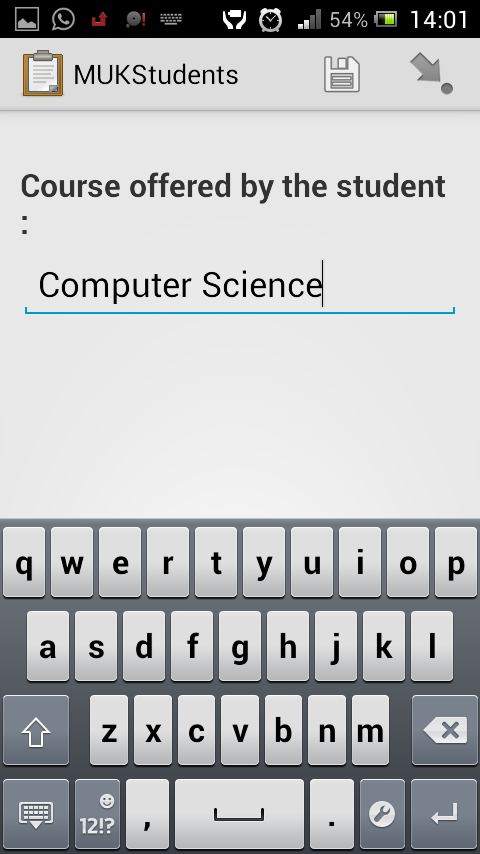
\includegraphics[width = 5cm , height = 8cm ]{course}
\graphicspath{{ODKprojectReport/}}
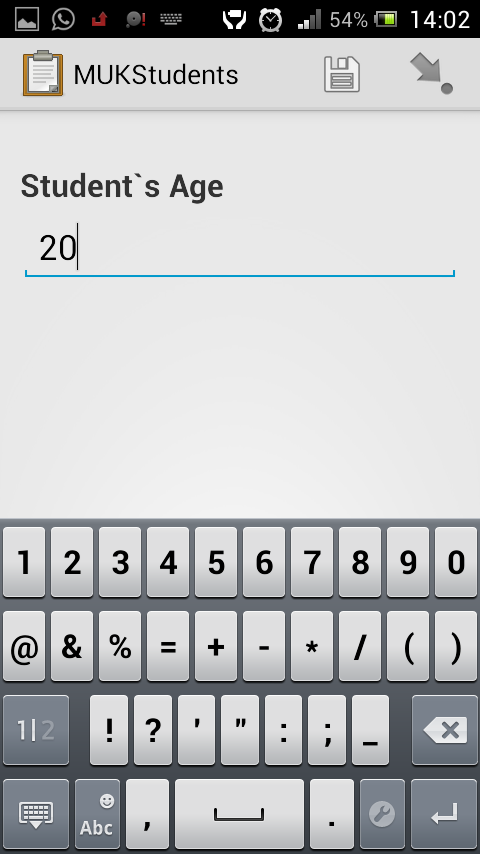
\includegraphics[width = 5cm , height = 8cm ]{age}
\graphicspath{{ODKprojectReport/}}
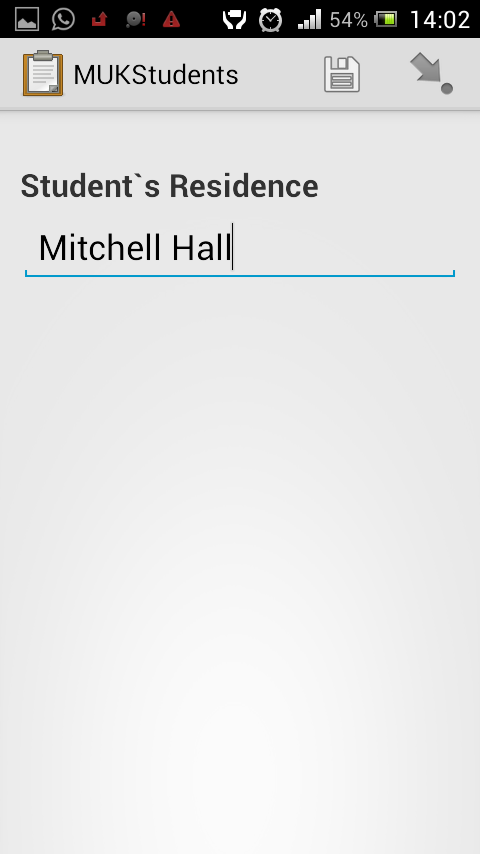
\includegraphics[width = 5cm , height = 8cm ]{residence}
\graphicspath{{ODKprojectReport/}}
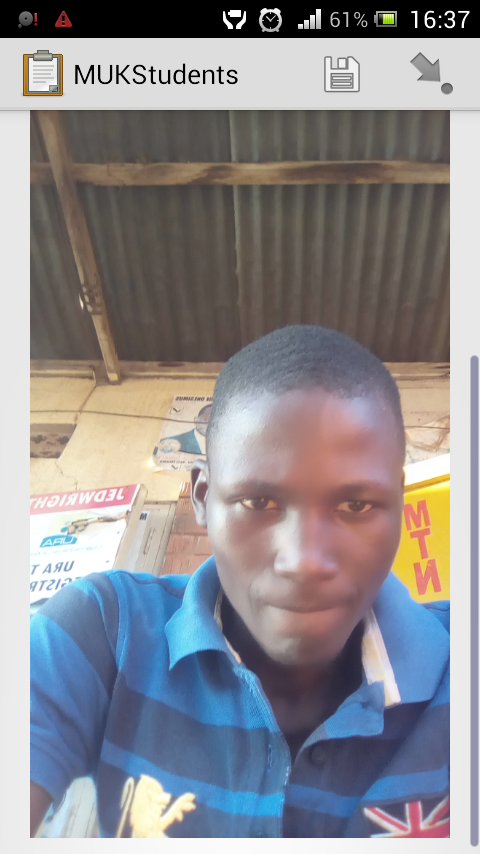
\includegraphics[width = 5cm , height = 8cm ]{image}
\graphicspath{{ODKprojectReport/}}
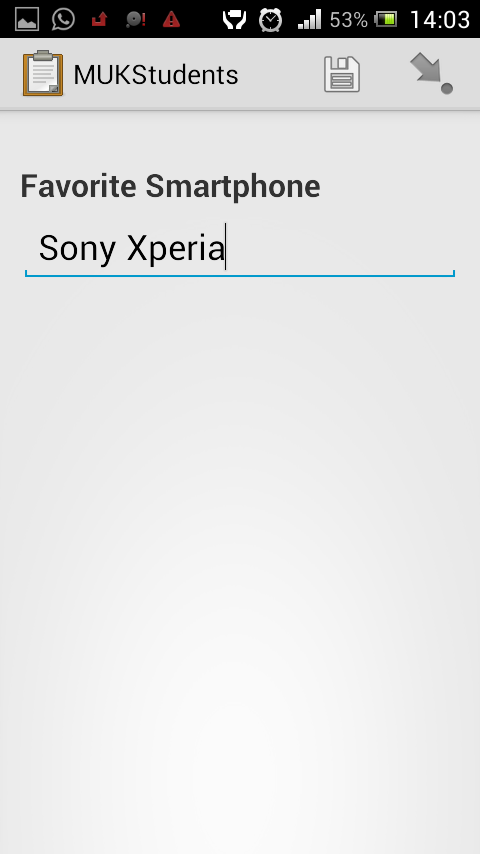
\includegraphics[width = 5cm , height = 8cm ]{favoriteSmartphone}



And it is summarisedin table 1 as shown in the table below :
\subsection{Table 1}

\begin{tabular}{|c|c|c|c|c|c|c|}
	
	
\hline	$NAME$ & COURSE & AGE & RESIDENCE & PHOTO & FAVORITE & LOCATION \\ \hline
\hline	$ Micheal$ &  CS &20&Mitchell&MIKE.jpg&SONY &LATITUDE 1 \\ \hline
\hline	$ Ronald$ &  MEC &21&Nsibirwa&Rona.jpg&HUAWEI &LATITUDE 2 \\ \hline
\hline	$ Tausi$ &  EDU &20&KAWEMPE&Tausi.jpg&Note1 &LATITUDE 3\\ \hline
\hline	$ Isaac$ &  CS &22&Gayaza&Isaac.jpg&HUAWEI P6 &LATITUDE 4 \\ \hline
\hline	$ Sandrah$ &  ELE &20&AFRICA&Sandrah.jpg&LG &LATITUDE 5\\ \hline
\hline	$ Joyce$ &  SE &20&Biira&Joyce.jpg&IPhone &LATITUDE 6\\ \hline
\hline	$ Patience$ &  BLISS &20&Complex&Patience.jpg&TECNO &LATITUDE 7 \\ \hline

	
\end{tabular}

\textbf{On the server, the information is stored as shown below}

\subsection{server table}
\graphicspath{{ODKprojectReport/}}
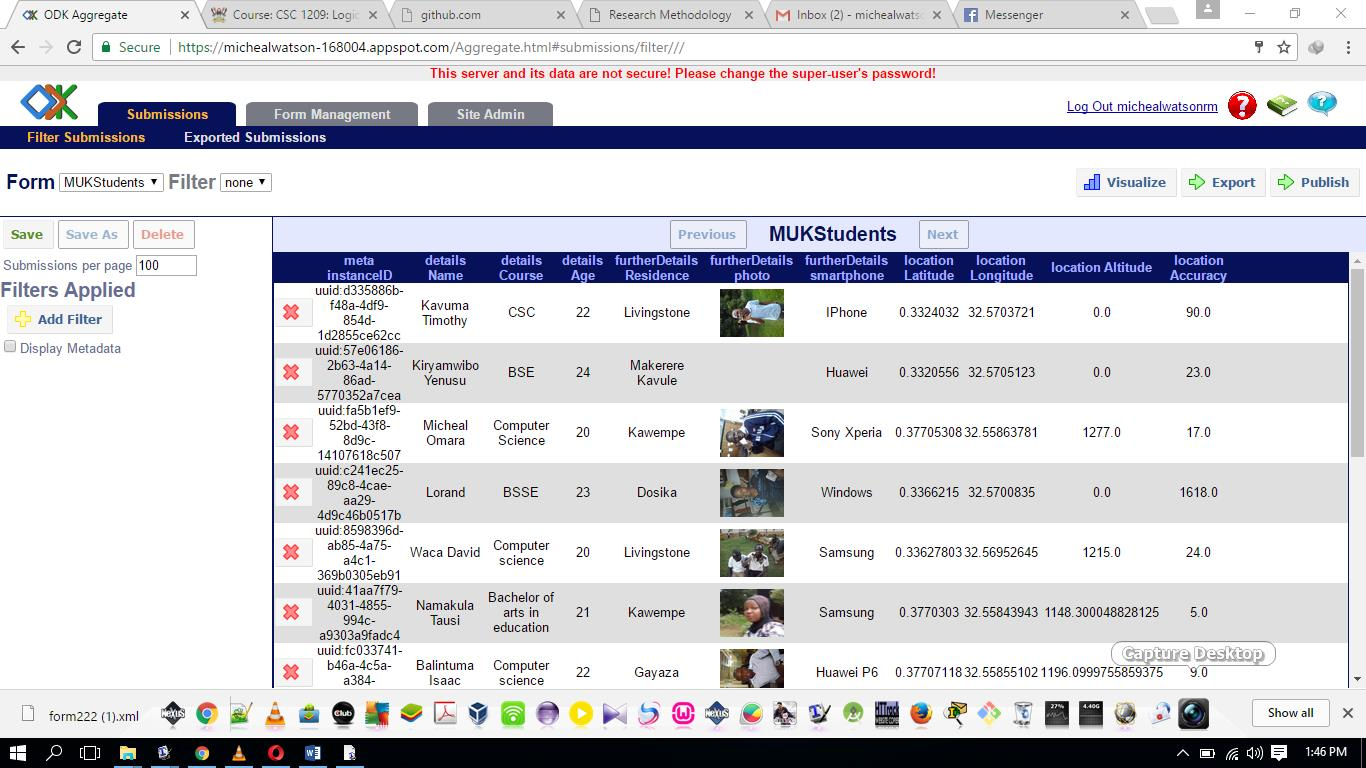
\includegraphics[width = 16cm , height = 10cm ]{Screenshot1}




\section{Conclusion}
Finally , the overall brand preferred by students is determined by getting a smartphone brand with the most frequency i.e : the smartphone appearing most in students` choices as data was collected.

\end{document}